\documentclass[a4paper]{article}

\usepackage{tecnico_relatorio}


\usepackage[hypcap]{caption} % makes \ref point to top of figures and tables
\usepackage{rotating}

\begin{document}
	\trSetImage{img/tecnico_logo}{6cm} % Logotipo do Técnico
	\trSetSubject{Arquitecturas Avançadas de Computadores}
	\trSetType{Laboratório III - Paralelização e Aceleração de um Programa}

	
	\trSetBoxStyle{0.3}
	
	\trSetAuthorNr{3}
	
	\trSetAuthors
	{
		\begin{center}
			Gonçalo Ribeiro

			73294
		\end{center}
	}{
		\begin{center}
			Miguel Costa

			73359
		\end{center}
	}{
		\begin{center}
			Rafael Gonçalves

			73786
		\end{center}
	}
		
	\trSetProfessor{Prof. Leonel Sousa}
	
	\trMakeCover
	
	\tableofcontents
	\pagebreak
	
	\section{Introdução}
	
	O objectivo do presente trabalho laboratorial é a aceleração e paraleliazação de um algoritmo de \textit{smoothing}. Foi dada a possibilidade de realizar este projecto recorrendo a instruções vectoriais ou utilizando um processador gráfico, sendo que se escolheu utilizar instruções vectoriais suportadas pela arquitectura Intel IA32e (MMX, SSEx, AVX). 
	
	O algoritmo de \textit{smoothing} consiste na obtenção de uma função aproximada, em que é filtrado todo o rído resultante da amostragem do sinal. Na \autoref{fig:fun_smoothing} estão representados dois gráficos, em que o primeiro demostra o sinal com ruído e o segundo a função resultante após se aplicar \textit{smoothing}.
	
		\begin{figure}[h]
			\centering
			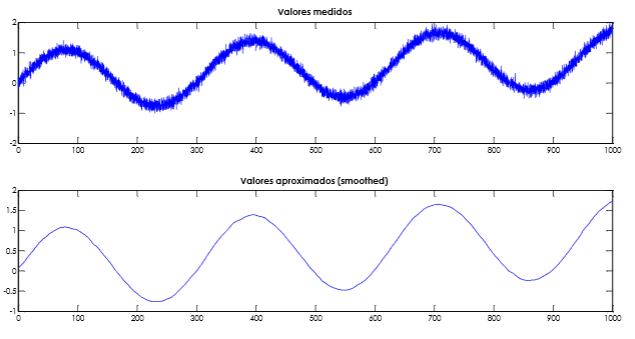
\includegraphics[width=1.\textwidth]{img/fun_smoothing}
			\caption{Resultado da aplicação de \textit{smoothing} a um sinal com ruído. }
			\label{fig:fun_smoothing}
		\end{figure}
		
	Para calcular o \textit{smoothing} foi fornecida a equação que permite calcular o valor aproximado $\hat{y}$$ _1$, $...$ , $\hat{y}$$ _{N-1}$, tendo em conta a função observada no domínio $x$$ _1$, $...$ , $x$$ _{N-1}$, dando origem aos pontos $y$$ _1$, $...$ , $y$$ _{N-1}$:
	
	\begin{equation}
		\hat{y}_i =  \frac{ \sum_{k=0}^{N-1} K_b (x_i, x_k ) y_k}{\sum_{k=0}^{N-1} K_b (x_i, x_k )} 
		\label{eq:smoothing_function}
	\end{equation}
	
	Onde
	
	\begin{equation}
		K_b (x_i,x_k)=exp\left(-\frac{(x-x_k)^2}{2b^2} \right)
		\label{eq:smoothing_kb}
	\end{equation}
	 	
	 	 
	Também é já fornecido um algoritmo (algoritmo 1) que ilustra um exemplo para calcular o resultado da função de \textit{smoothing}.
	
	
	\section{Performance}
	
	\section{Testes} 
		
	\section{Conclusão}

\end{document}
